%!TEX root = thesis.tex

%:-------------------------- Preamble -----------------------

% Three languages are supported, which will be reflected in the logo on the front page. Pass the appropriate language
% specified as a class option to uit-thesis. Passing any other languages supported by babel will result in the default
% language on the frontpage. If no language is passed, the default is selected.
%  - USenglish (default)
%  - norsk
%  - samin
% The frontpage comes in two variants, Master's thesis and PhD. Master is default, use classoption 'phd' for the PhD version.
\documentclass[USenglish]{uit-thesis}
\renewcommand{\bibname}{References}
% Lorem ipsum
\usepackage{lipsum}
\usepackage{appendix}
\usepackage{amsthm}
\usepackage{hyperref}
\usepackage{tikz}
\usepackage{pgf-umlsd}
\usepackage{float}
\usepackage{listings}
\usepackage{caption}
\usepackage{subcaption}
\usepackage{amsmath}
\usepgflibrary{arrows}
\usepackage{listings}

\usepackage{glossaries}

\newtheorem{defs}{Definition}

\makeglossaries

% Add external glossaryentries

\loadglsentries{acronyms}

\newglossaryentry{thesis}
{
  name=thesis,
  description={
    },
}
\newglossaryentry{lage}
{
  name={long ass glossary entry},
  description={
  },
}


\newcommand{\listdefinitionname}{My list of definitions}
\newlistof{definition}{def}{\listdefinitionname}
\newcommand{\definition}[1]{%
  \refstepcounter{definition}%
  \par\noindent\textbf{The Definition~\thedefinition. #1}%
  \addcontentsline{def}{definition}
    {\protect\numberline{\thechapter.\thedefinition}#1}\par%
}


\begin{document}
\renewcommand{\bibname}{References}
%:-------------------------- Frontpage ------------------------

% \title{Understanding Digital Currencies and Blockchain}
\title{Master Thesis title}
\subtitle{subtitle}			% Optional
\author{Enrico Tedeschi}
\thesisfaculty{Faculty of Science and Technology \\ Department of Computer Science}
\thesisprogramme{Master Thesis in Computer Science}
%\ThesisFrontpageImage{img/}	% Optional

\maketitle

%:-------------------------- Frontmatter -----------------------
\frontmatter

%\begin{dedication}
%Dedication here
%\end{dedication}

%\begin{epigraph}
%\epigraphitem{Simplicity is prerequisite for reliability.}{Edsger Dijkstra}
%\epigraphitem{Beware of bugs in the above code;\\I have only proved it correct, not tried it.}{Donald Knuth}
%\end{epigraph}

\begin{abstract}
\label{sec:abstract}

\end{abstract}

%\begin{acknowledgement}
%
%\end{acknowledgement}

\tableofcontents

\listofdefinition

%:-------------------------- Mainmatter -----------------------
\mainmatter
\chapter{Introduction}
\label{chap:introduction}

\section{Problem Statement}
\label{sec:probdefinition}

%\begin{quote}
%\emph
%{applications can control available bandwidth by paying mining fees.}
%\end{quote}


\section{Method / Context}
\label{sec:method}

\section{Outline}
\label{sec:outline}
%This chapter introduces the Blockchain, blocks, mining, fee and other key words related to
%decentralized digital currencies. Chaper~\ref{chap:techback} gives a detailed explanation
%on the main aspects of this new technology and how decentralized
%cryptocurrencies work. It will talk about consensus protocol, data structure, mining
%process, gas, fees and proof of work. Chapter~\ref{chap:expsetup} explains how the blockchain
%analytics system was designed and implemented, which data are
%taken into consideration and why and also how data are retrieved and
%organized into text files. Chapter~\ref{chap:evaluation} talks about the
%evaluation and the results of the data analysis. It shows the plots generated with some
%consideration and the comparison between the expected results from the Bitcoin blockchain.
%Plus, prediction models obtained with statistical analysis are showed.
%Finally, Chapter~\ref{chap:conclusion} includes future implementation of the system,
%possible development of this project and conclusions of the overall work.

%TODO: PREVIOUS WORK -- WORKING ON THIS CHAPTER
\chapter{Related Works}
\label{chap:prev_works}
This chapter summarizes the most relevant papers or works that talks about Bitcoin,
decentralized cryptocurrencies, concepts behind them and statistical analysis on the
blockchain. In a previous paper that we wrote~\cite{Tedeschi:2016:PBB}, we enhanced the
importance of paying for having a certain bandwidth in the Bitcoin network. A paper
from Peter~R.~Rizun~\cite{Rizun:2015:blocksizelimit}, explains how a rational Bitcoin
miner should select transactions from his node mempool, when creating a new block,
in order to maximize his profit. Analysis on the blockchain in matter of
scalability is showed in the Position Paper of Kyle Croman~\cite{croman2016}, they
analyze how fundamental bottlenecks in Bitcoin limit the ability of its current peer-to-peer
overlay network to support substantially higher throughputs and lower latencies. We are
going to test the throughput as well, comparing it with the one showed in this paper.

\section{A Transaction Fee Market Exists Without a Block Size Limit}
\label{sec:rizun}
This paper shows how a Bitcoin miner should select transactions from his node's mempool,
when creating a new block, in order to maximize his profit in the absence of a block size limit.
\emph{Block space supply curve} and \emph{mempool demand curve} are explained, and the
paper shows how the supply and demand curves from classical economics are related to the
derivatives of these two curves.


\chapter{Technical Background}
\label{chap:techback}
%This chapter will give a detailed explanation about decentralized digital
%currencies, explaining all the main concepts and key words that you should know when
%you read about cryptocurrency. 	The differences between centralized
%and decentralized cryptocurrencies are discussed, enhancing their main
%characteristics, pros and cons. Concepts such as blockchain, 
%proof of work, state, block, transaction, and gas fee
%are described and discussed.



%\definition{An \emph{eletronic coin} is a chain of digital signatures.
%Each owner transfers the coin to the next by digitally signing a hash of
%the previous transaction and the public key of the next owner and adding
%these to the end of the coin.}




%\definition{A \emph{transaction} (formally, $T$) is a single
%	cryptographically-signed instruction constructed by an actor with the scope of giving
%	money to someone else in the network.}


\chapter{Blockchain Analytics System}
\label{chap:expsetup}
%In order to understand digital cryptocurrencies systems,
%to test and make experiments on the blockchain, a complete data analytic
%system was designed and implemented. This chapter will explain how the
%blockchain analytics system on Bitcoin was implemented,
%starting from its architecture until the \gls{api}
%used and then how data are processed and manipulated.

\section{Blockchain Data Sources}
\label{sec:apis}
%There are many websites that observe and make analysis on the existing blockchains. The most
%popular websites for Bitcoin and Ethereum blockchain analysis are \url{blockchain.info}\,\cite{bitcoin_blockchain}
%for Bitcoin, \url{etherscan.io}\,\cite{ethereum_bc_analysis} and \url{etherchain.org}\,\cite{ethereum_blockchain}
%for Ethereum.
%Remote \gls{api} on the Bitcoin blockchain could be found at \url{blockchain.info}
%in the \gls{api} section. These are \gls{api} to retrieve data directly from
%the website and they can be used in a Python application simply as a HTTP request/response.
%The system we implemented retrieves data from the Bitcoin blockchain, using the \gls{api}
%provided from \url{https://github.com/blockchain/api-v1-client-python}. This \gls{api} is well suited
%for Python and provides a nice access to the Bitcoin blockchain, allowing the retrieval
%of all the information stored in a block and in a transaction.
%
%In the api-v1-client-python mentioned above, the class containing the
%structure of a block and transaction, used for data retrieval and
%analysis is \emph{blockexplorer.py}. The object structures of a block and a
%transaction in Python language are represented in Appendix~\ref{lst:block},~\ref{lst:transaction}.
%Furthermore, in Appendix~\ref{lst:block-json} is showed a JSON representation of the block which is
%returned from the \gls{api} call.

\section{System Architecture}
\label{sec:implementation}

%\begin{figure}[h]
%	\centering
%	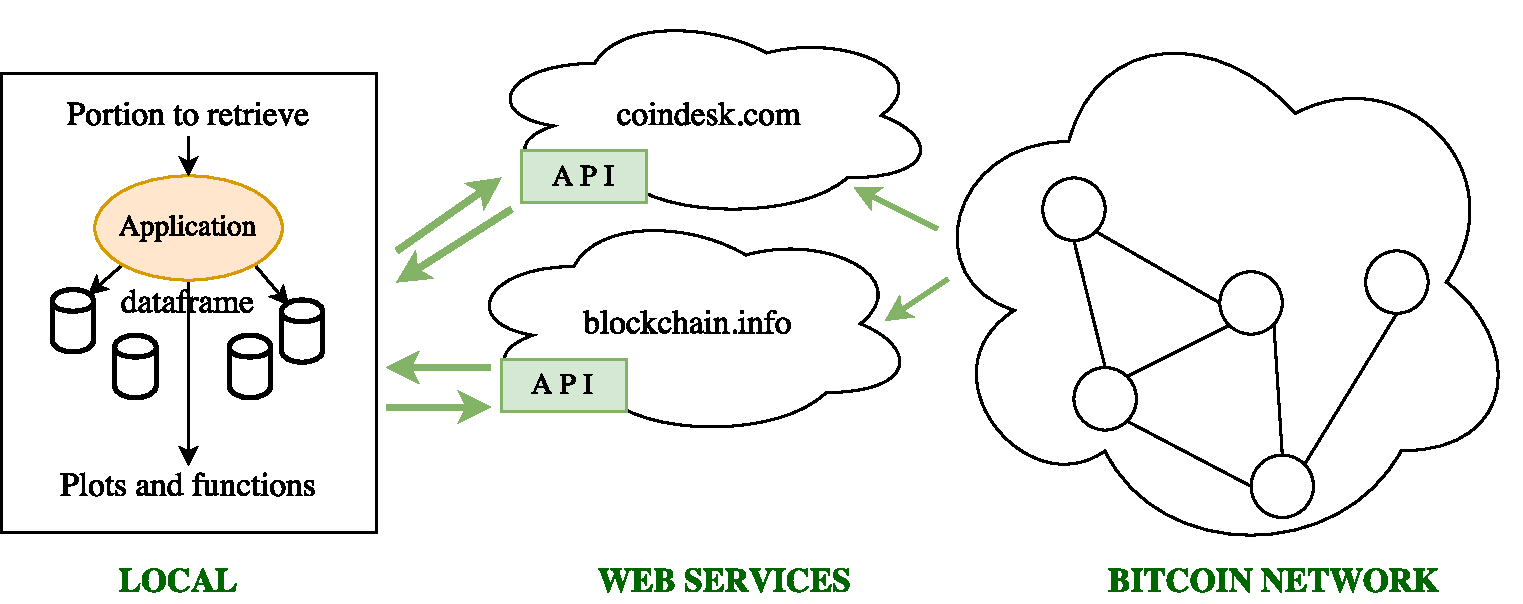
\includegraphics[width=1\textwidth]{img/architecture}
%	\caption{Architecture of the developed system for blockchain analysis.}
%	\label{fig:architecture}
%\end{figure}
%
%The architecture of our blockchain analytic system is showed in Figure~\ref{fig:architecture}. The system 
%is run mainly locally, importing Bitcoin \gls{api} and using them for data retrieval to the
%local system. The website \url{blockchain.info} provides \gls{api} to be used remotely with an
%HTTP request, and they can be easily integrated in the application with a HTTP
%request/response mechanism. The website \url{blockchain.info} contains all the information
%concerning the Bitcoin blockchain and it could be queried both through Python \gls{api}
%and web \gls{api}. This website is monitoring 24-7 the blockchain, producing graphs and
%statistical analysis on the data observed in the real decentralized network. The local
%application is monitoring these data as well, producing graphs that are not taken into
%consideration from the \url{blockchain.info} website, using a finer granularity that represent
%the data. Moreover, the application generates three text files:
%\begin{description}
%	\item [blockchain.txt:] text file containing information about the portion
%	of the blockchain retrieved, including block hash, height, size, fee and
%	time for each block. These data are important for the later analysis and the file is structured like the following:
%	\begin{lstlisting}
%hash:		block_hash
%epoch:		block_epoch
%creation_time: 	time_mining_block (s)
%size: 		block_size (byte)
%fee: 		block_fee (satoshi)
%height: 	block_height (block_number)
%bandwidth: 	read_bandwidth (MB/s)
%transactions: 	number_transactions_in_block
%avgttime: 	avg_tr_time (s)
%	\end{lstlisting}
%	\item [mining\_nodes.txt:] text file containing all the IP addresses of mining nodes or pools
%	concerning the blocks in the file "blockchain.txt".
%	\item [nodes\_in\_the\_network.txt:] text file containing all the IP addresses involved in relaying transactions
%	in the network.
%\end{description}
%
%The application for blockchain analysis is implemented in the file  \emph{observ.py}, it provides
%to call \gls{api} functions and to generates all the output files. A small
%example of how the \gls{api} calls work in the system is showed in Appendix~\ref{lst:api-python}.
%Our blockchain analytic system was implemented on a MacBook Pro with MacOS Sierra \emph{v$10.12.1$},
%with a $2.8$\,GHz Intel Core i$7$ processor and $16$\,GB~$1600$\,MHz DDR3 of RAM, using
%JetBrains PyCharm (\emph{v$2016.2.3$}) software as text editor and \emph{Python v$2.7.12$}
%as programming language.

\subsection{Data Retrieval}
\label{sec:data_retrieval}
%Data in the blockchain can be retrieved in different ways: blocks can be added to
%the top of the file, so the most recent blocks are fetched, or appended to the last element,
%so the blockchain is analyzed even further in the past.
%To fetch the most recent block the method showed in Appendix~\ref{lst:api-python}
%is used. First, the latest block is fetched, then from the previous is retrieved and so on.
%The latest block is saved with a structure showed in Appendix~\ref{lst:latest-block}.
%When data are appended to the last block, instead, is necessary first to get the hash
%from the last element in the "blockchain.txt" file, then the last block is retrieved
%using the method \emph{get\_block(hash)} provided from the Bitcoin \gls{api}.
%The implementation of the append is found in Appendix~\ref{lst:append-block}.
%
%Blockchain is meant to be ordered linearly and every block should have its predecessor,
%for this reason blocks are collected in a way that there will not be any gap in the local blockchain, and
%if the number of blocks that the user tries to fetch is less than the blocks
%already added to the global blockchain, then would be impossible to add any new block.
%In this case a better option would be to \emph{update} the local blockchain (-u command, view the application
%usage~Appendix~\ref{lst:usage}), which means that the right number of blocks that will complete
%the local chain will be automatically retrieved. A simplified scheme to add blocks on
%the local blockchain is showed in Figure~\ref{fig:blockchain-scheme}. To guarantee that the order is
%respected and the blockchain is saved locally in a correct way, a validity check is done every time
%the application is executed. This check verifies that
%each block in the local blockchain has the right predecessor by controlling that there is a
%diminishingly height by one going from one block to another (Appendix~\ref{lst:check}).
%\begin{figure}[h!]
%	\centering
%	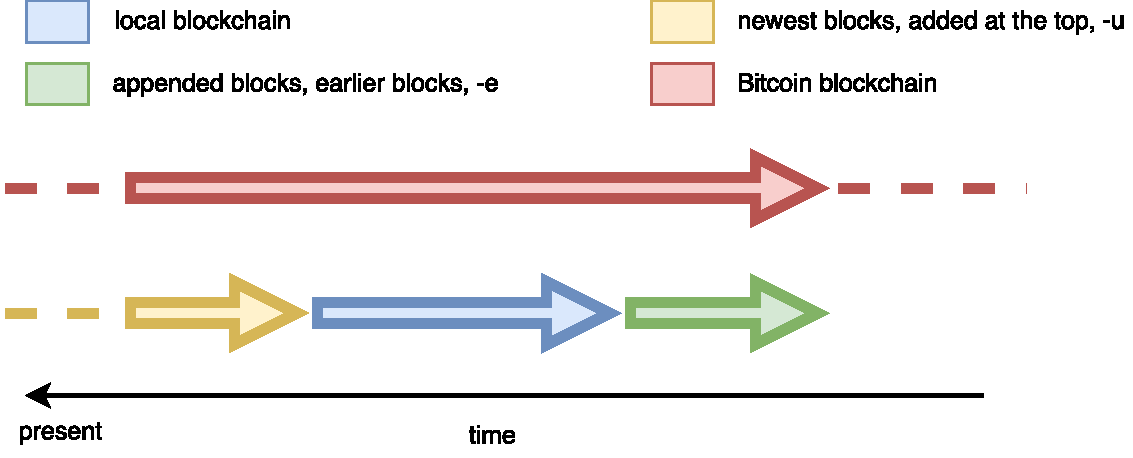
\includegraphics[width=1\textwidth]{img/blockchain-scheme}
%	\caption{Scheme that shows how blocks are written in the local blockchain file.}
%	\label{fig:blockchain-scheme}
%\end{figure}
%
%Once blocks are retrieved a \emph{file.write} is performed. Writing on blockchain.txt
%can be done by appending blocks at the end or adding them at the beginning
%of the file. As Appendix~\ref{lst:file-write} shows, the adding part is much more
%complicated since the file needs to be deleted and then written again for each block
%that needs to be added.
%As showed in Chapter~\ref{sec:implementation} before plotting and getting any
%kind of information from the data, they are evaluated and manipulated for our purposes.
%The blockchain.txt file saved, contains information about block hash, height, size, fee, epoch
%time, creation time, read bandwidth, number of transactions and the average transaction
%visibility time (average write bandwidth for a block). Of course not all these data are
%provided from the Bitcoin \gls{api}, so they are calculated and manipulated runtime, then saved in the text file.

\subsection{Data Manipulations}
%Data manipulation is done both before (to save data correctly) and after
%(to plot data correctly) data are collected in the
%blockchain.txt file. Once data are retrieved and saved, they are ready to
%be manipulated in a way that the right and needed information can get
%out of them.
%
%Each block $B$, retrieved from the blockchain.txt file, has the following attributes.
%The \emph{hash}, $B.hash$, is a string containing the 256-bit hash for the block $B$.
%The \emph{epoch}, $B.epoch$, which represents the epoch time when the block was created and
%got visible in the blockchain. This means that the retrieval time is in seconds,
%starting from the epoch which is $1^{st}$ January $1970$ at $00$:$00$:$00$. The time is
%always collected as seconds and if needed, is converted in minutes and
%hours and saved in other lists.
%The \emph{size}, $B.size$, is represented in bytes, so every time that MB are needed, the
%size is divided by $10^6$. The growth of the blockchain is represented in GB and
%the block size and the read/write bandwidth in MB.
%The \emph{fee}, $B.fee$, represents how much the miner of the block get in satoshi~(Appendix~\ref{app:terminology})
%to mine a certain block $B$. To be more readable, plots using satoshi are converted in BTC.
%The \emph{creation time}, $B.creation\_time$, is represented in seconds, and it tells how much time
%a block needs to be mined.
%The \emph{number of transactions}, $B.transactions$, tells how many transactions are accepted and
%stored in the block $B$.
%The \emph{write bandwidth}, $B.avgttime$, is the average of the all transactions acceptance time
%in a certain block and it is measured in seconds. A transaction $T$ is accepted when the block $B$ is
%created so the $read\_bandwidth_T$ will be:
%\begin{equation}
%\label{eq:read_bandwidth}
%read\_bandwidth_T = B.epoch - T.time
%\end{equation}
%where $T.time$ is the epoch representing the transaction request.
%
%The read bandwidth is calculated as showed in Appendix~\ref{lst:read-bandwidth}.
%Start time and end time are calculated before and after the block retrieval call, with
%the function \lstinline|datetime.now()|. Time is manipulated to be showed in seconds and then
%the ratio to get the bandwidth between $MB/s$ is done and the value is appended
%in a list that will be written in the file.
%
%The write bandwidth is calculated first for each transaction in the block, as the
%Appendix~\ref{lst:get-transaction-time} shows, and then an average is done
%for each block and returned as a data to append in a list containing
%all the write bandwidths for each block retrieved, this data is written in the
%blockchain.txt file as \emph{avgttime}.
%
%To represent the growth of the blockchain, a growing time and size list needs
%to be generated. Assuming that a block is represented with $B$ and its creation time is $B.epoch$,
%we define the block creation time in the following way:
%\begin{flalign}
%\label{eq:creation_time}
%creation\_time_n = \begin{cases} 0, & \mbox{if } n = 0\\ B.epoch_n - B.epoch_{n-1}, & \mbox{if } n > 0 \end{cases}&&
%\end{flalign}
%where $B.time_{n-1}$ is its predecessor.
%The growth of the blockchain is calculated by comparing the sum of the creation time
%and the sum of the block size each time, generating ever growing lists as shows the Appendix~\ref{lst:growing-lists}.
%Assuming that $B.size$ is the block size, then:
%\begin{flalign}
%\label{eq:growing_time}
%&growing\_time_n = \begin{cases} 0, & \mbox{if } n = 0\\ creation\_time_n + creation\_time_{n-1}, & \mbox{if } n > 0 \end{cases}&&
%\end{flalign}
%and:
%\begin{flalign}
%\label{eq:growing_size}
%&growing\_size_n = \begin{cases} 0, & \mbox{if } n = 0\\ B.size_n + B.size_{n-1}, & \mbox{if } n > 0 \end{cases}&&
%\end{flalign}
%where $growing\_time$ is the list containing the sums of the creation time every time that a new
%block is created and $growing\_size$ is the list containing the size of the blockchain
%as every block is added.
%
%One of the reason why Python was chosen as a programming language is because
%data structures are easy to manage and with a Python list you can change the whole
%data in it using only one line of code~(Appendix~\ref{lst:python-list}). It is very easy indeed to swap an entire
%list from minutes to seconds, from seconds to hours and vice versa. Furthermore,
%mature API bindings do exist for Python, and it is a very intuitive language with a lot
%of useful libraries for data manipulation and plotting.

\subsection{Methods}
%An UML diagram of the main methods used in the application is represented in
%Figure~\ref{fig:uml_sequence_diagram_application}.
%The application usage is described in Appendix~\ref{lst:usage} and the main
%methods in the systems are:
%\begin{description}
%	\item [\emph{get\_blockchain(n, [hash])}:] method that retrieve the blocks
%	from the Bitcoin blockchain and saves them in lists that will be the input
%	of the write\_blockchain() method. If the attribute hash exists then the retrieval
%	starts from that hash and not from the latest block created in the Bitcoin blockchain.
%	Part of it is represented in Appendix~\ref{lst:append-block}.
%	\item [\emph{write\_blockchain(<lists to write>, [to\_append])}:] method that takes lists in input and write them into a file,
%	according to the parameters that it gets. If to\_append is True, then data are appended otherwise are added, like
%	shows Appendix~\ref{lst:file-write}.
%	\item [\emph{get\_list\_from\_file(attr)}:] this method is probably one of the most important concerning data
%	manipulation. It creates a list, given an attribute as input. Such attribute is a block information stored in the
%	local blockchain and the list generated contains all the values from every block, concerning that
%	particular  attribute.
%	Lets say that informations about the block hash want to be analyzed, then it would only be necessary
%	to make a call to this method giving as attribute the string \emph{"hash"}, like showed in Appendix~\ref{lst:get-data-from-file}.
%	In that way the return list will contain hashes about all the blocks retrieved with the most recent hash In list[$0$].
%	Regular expression\,\cite{Aho:1992:FCS} is used to analyze the file and read from it, in this way is possible
%	to interact with the saved data and get informations from them. This method allows the
%	function plot\_data() to easily display statistics.
%	\item [\emph{plot\_data(d, n, [r], [s], [e])}:] this method gets the data from the
%	txt file and then plots all the information retrieved using Matplotlib libraries\,\cite{matplotlib}. It has
%	a description, $d$, a number of the plot, $n$, and an optional parameter about the
%	regression, $r$. It also has the possibility to chose the range of the plot with the start, $s$, and end, $e$,
%	parameters. If in the local txt file are present $10000$ blocks, is possible to call the method with
%	$start=7000$ and $end=9000$, in that way only the blocks in between $7000$ and $9000$
%	will be taken into consideration for the plots. In that way is easier to verify if the predictions on
%	the blockchain growth were accurate or not.
%\end{description}
%
%\begin{figure}[h]
%	\centering
%	\begin{sequencediagram}
%		\newthread{m}{main()}
%		\newinst{gb}{get\_bc()**}
%		\newinst{wb}{write\_bc()**}
%		\newinst{bi}{bc.info**}
%		\newinst{pb}{plot\_data()*}
%		
%		\begin{callanother}{m}{1}{gb}{}
%			\mess{gb}{}{bi}
%			\mess{bi}{get data}{gb}
%				\begin{callanother}
%				{gb}{2}{wb}{}
%			\end{callanother}
%		\end{callanother}
%
%		\begin{callanother}
%			{m}{3}{pb}{}
%		\end{callanother}
%		
%	\end{sequencediagram}
%	\begin{enumerate}
%		\item call the method \emph{get\_blockchain()} for blocks retrieval
%		\item write data in the txt.file
%		\item call the plot function for data plotting
%		\item[*] not every function or method is showed in the diagram, the
%		function plot\_data() calls some methods for data management.
%		\item[**] the word blockchain has been replaced with the shortcut
%		bc
%	\end{enumerate}
%	\caption{UML sequence diagram of how the application works, where
%		the threads are the methods implemented in \emph{observ.py} file.}
%	\label{fig:uml_sequence_diagram_application}
%\end{figure}
%
%
%The \emph{main()} method provides to call the others and if the
%\gls{grasp} principle is followed\,\cite{Larman:2004:AUP}, then this method would be
%the controller, dispatching calls to other methods for collecting, analyzing and plotting
%data.
%
%Not all the methods implemented in the system are listed above. Some include
%data management or check of the blockchain status, such as converting the
%epoch time in date time format $DDMMYYYY$, get the number of blocks currently
%present in the local blockchain or create the growing size and time lists.
%The method \emph{add\_mining\_nodes(block)} concerns the creation of a file containing
%mining nodes and a file containing nodes involved in every transaction. The second
%one are the nodes that rely transactions in all the block retrieved.
%This means that for each block given in input, every transaction is analyzed, and if the node
%relying this single transaction is not in the file yet, then the IP for this node is added to it.

\section{Version Control}
\label{sec:versioncontrol}
%For the version control on the source code, a public \emph{git} repository at:
%\url{https://github.com/ted92/blockchain.git} was created. Git version \emph{2.6.4}
%is used in the local environment and every significant update is pushed to the
%repository to keep an history of all the changes and how the application was
%developed.

\chapter{Blockchain Observations}
\label{chap:evaluation}
%In this chapter we present observations of the Bitcoin blockchain captured by the
%analytics system outlined in Chapter~\ref{chap:expsetup}. 
%To evaluate our problem definition in Chapter~\ref{sec:probdefinition}, we focus on consideration related to 
%read/write bandwidth, the growth of the blockchain, and the relation between the fee paid and the bandwidth achieved.
%The evaluations are made by analyzing the plots generated in the plot/
%folder using Matplotlib\,\cite{matplotlib}. A large number of test has been
%done, considering always a different number of blocks fetched, at different time.
%%TODO: put the following also in the abstract and in the introduction
%We show that the fee paid is related to the amount of time that a block needs to be mined and be visible in the whole network.
%This affects average bandwidth available to an application.

\section{Blockchain Growth}
\label{sec:blockchain_growth}
%To understand the capacity of the Bitcoin blockchain, we first study
%its size and how it grows over time. For this, we've been analyzing the blockchain
%periodically from the $21^{st}$~September~$2016$ until the $11^{th}$~December~$2016$
%using the system outlined in Chapter~\ref{chap:expsetup}. The plotted growth is
%shown in Figure~\ref{fig:growth_blockchain}. We observe that the blockchain size grows
%of $10,139$\,GB in $1940$ hours. That means a bandwidth usage of $\sim5,22$\,MB per hour. 
%Our findings are inconsistent with the observations from
%$2014$~\cite{ethereum_white_paper} that observed a growth
%of~$\sim$1\,MB per hour. Our observations indicate that the growth of the
%Bitcoin blockchain is $5x$ times bigger than it was expected in 2014 and we
%believe that a more accurate model for the blockchain growth can be created.

%\begin{figure}[h!]
%	\centering
%	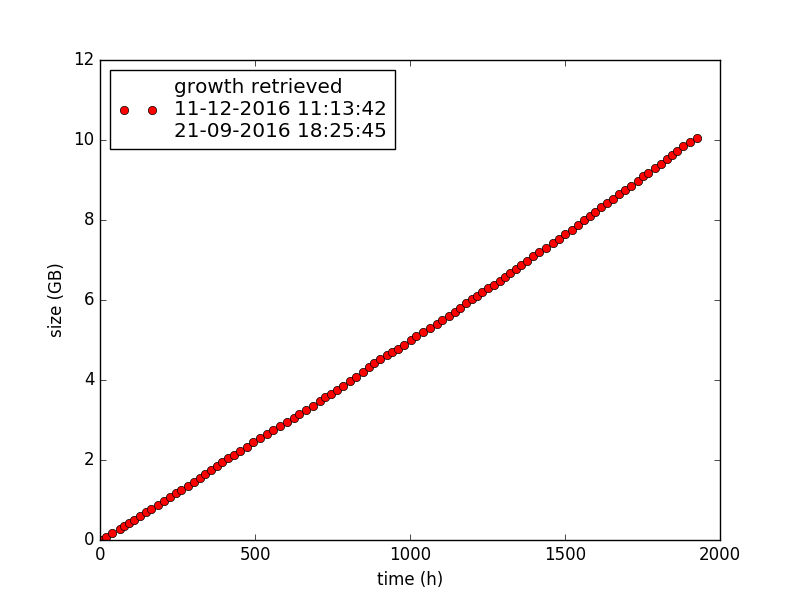
\includegraphics[width=1\textwidth]{img/growth_blockchain}
%	\caption{The Bitocin blockchain growth according to our analytics system.
%		12091 blocks are fetched between the $21^{st}$~September~$2016$ and the $11^{th}$~December~$2016$.}
%	\label{fig:growth_blockchain}
%\end{figure}

%From the plot in Figure~\ref{fig:growth_blockchain} the growth seems to be linear.
%However, evaluations made using polynomial interpolation on these data show that the growth has,
%even if small, a coefficient on the $x^2$. Our hypothesis is that the non-linear growth
%is due to a small increment of the block size during the years.
%To prove this, two different measurements have been done to our local blockchain, showed in
%Figure~\ref{fig:size_comparison}. The first one, Figure~\ref{fig:size_comparisonA},
%considers $1000$ blocks fetched from $22^{nd}$~September~$2016$ until
%$28^{th}$~September~$2016$, shows that the block size tends to be $1$\,MB
%but with quite a lot of blocks having also different sizes. While the latest one, in Figure~\ref{fig:size_comparisonB},
%shows that almost every block out of $1000$ are tending to the $\sim1$\,MB size, having only few blocks under
%the $1$\,MB "line". The second measurement was evaluated between $04^{th}$~December~$2016$ and
%$11^{th}$~December~$2016$.
%Furthermore, if the blocks from $2009$ in the blockchain are analyzed, their sizes tend
%to be~$\sim$200\,kB while in this last months of analysis, December~$2016$ the block size tend to be of $\sim1$\,MB.
%This brings us to believe that the average block size is growing with time,
%hence the blockchain growth is not linear as previously claimed\,\cite{ethereum_white_paper}. 

%\begin{figure}[H]
%	\centering
%	\begin{subfigure}{1\textwidth}
%		\centering
%		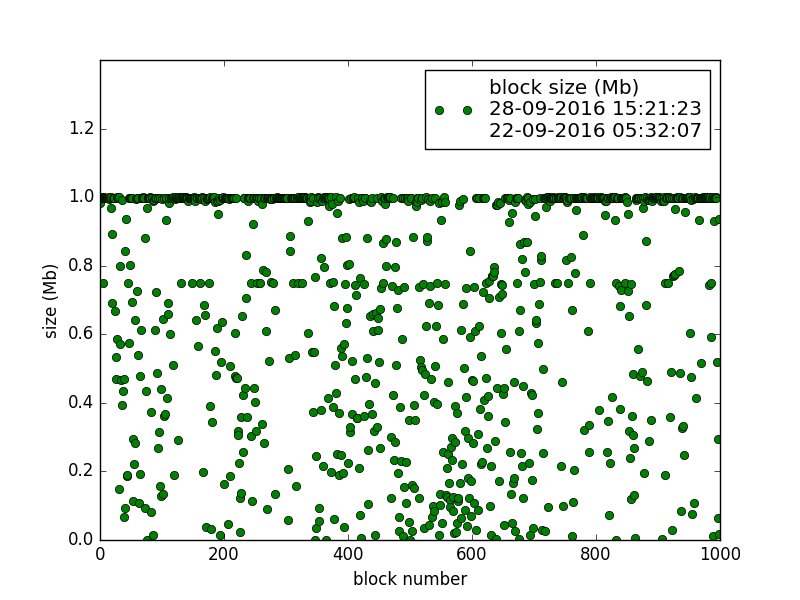
\includegraphics[width=1\linewidth]{img/byte_per_blockA}
%		\caption{Late September~$2016$.}
%		\label{fig:size_comparisonA}
%	\end{subfigure}
%
%	\begin{subfigure}{1\textwidth}
%		\centering
%		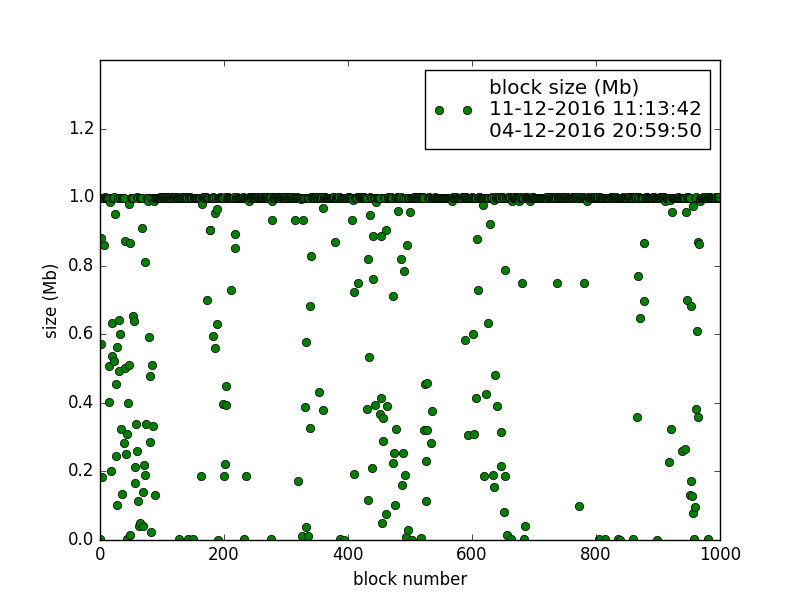
\includegraphics[width=1\linewidth]{img/byte_per_blockB}
%		\caption{Mid December~$2016$.}
%		\label{fig:size_comparisonB}
%	\end{subfigure}
%	\caption{Size comparison of $1000$ blocks with more than 2 months of gap.}
%	\label{fig:size_comparison}
%\end{figure}

\section{Retrieval Block Time}
%\label{sec:retrieval_block_time}
%The biggest problem analyzing the blockchain was that the \gls{api} allows to
%retrieve only one block per time, making the block fetching incredibly slow. This
%is the reason why the block retrieval is kept separate from the analytics part,
%in that way is possible to fetch a fewer number of blocks, adding them time
%by time and at the end make analysis on them.
%In Figure~\ref{fig:bandwidth} the read bandwidth for each block retrieval is
%represented. As said before, the problem of a single-block-fetch affects
%drastically the latency, and then the read bandwidth as well,
%taking an average of~$\sim1$\,seconds to retrieve a
%single block, and in some blocks the read bandwidth is even less than $0,5$\,MB/s.

\section{Block Analysis}
\label{sec:block_analysis}
%The most important attributes of blocks are their size, their creation times, and the
%number of transaction in each individual block. In this section, we will compare this
%three attributes to see if there could be any relation between them.
%The plot in Figure~\ref{fig:efficiency} shows that the block size tend to be $\sim1$\,MB.
%This observation does not depend on how many
%transactions it contains or how much time it needed to be mined.
%No relation also was found between the number of transactions in a block and the block
%creation time. In the Figure~\ref{fig:efficiency} sometimes the blue line (block creation time)
%follows the red one (number of transactions in one block), so if one grows then also the
%other gets higher, but in other cases there is a reverse dependence, so if the number of
%transactions grows, the block creation time decreases. This unpredictability
%is good for the security of the blockchain, since malicious node cannot find any dependence
%on the data which are more representative for a block.
%
%Figure~\ref{fig:time_per_block} shows the creation time for each block,
%retrieving blocks from the Bitcoin blockchain between the $4^{th}$
%and $12^{th}$~December~$2016$. How mining works is described in
%Chapter~\ref{sec:mining} and according to the difficulty, which is constantly adjusted, a
%block should be mined every $10$\,minutes\,\cite{bitcoinmining}. This claim
%tend to be verified for most of the blocks, however, there are too many peaks with a
%creation time of $20$\,minutes (which is already the double) until $40$\,minutes, up to even
%$80$\,minutes per block. When a block takes $80$\,minutes to be mined, it will affect the
%visibility of all the transactions in that block, mining the consistency of the system, since, in
%an average scenario a sender expects that its transaction is visible after $\sim8$-$15$\,minutes.
%\begin{figure}[h]
%	\centering
%	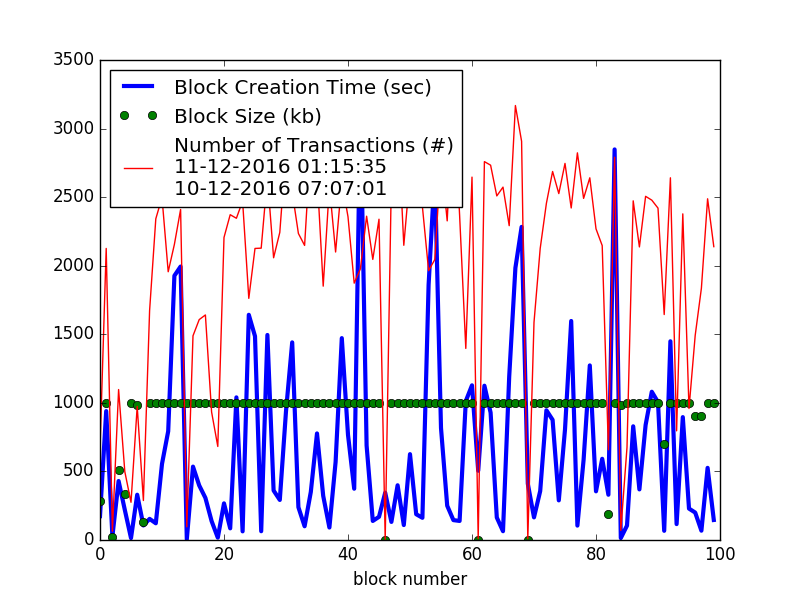
\includegraphics[width=1\textwidth]{img/efficiency(100)}
%	\caption{Relation between block creation, block size and number
%		of transaction in a block. Measurement done on
%		Bitcoin blockchain from $10^{th}$~December~$2016$ until
%		$11^{th}$~December~$2016$.}
%	\label{fig:efficiency}
%\end{figure}

\section{Bandwidth}
\label{sec:bandwidth}
%As explained in Chapter~\ref{sec:method}, the bandwidth represents the speed,
%in MB/s, for a transaction to be visible and accepted (write bandwidth), and the speed, always in MB/s, that
%a node has while fetching this block (read bandwidth). The Figure~\ref{fig:bandwidth}
%shows that the read bandwidth while monitoring the blockchain for more than 2 months,
%has an average speed of $\sim1$\,MB/s and it doesn't go faster than $9$\,MB/s. This
%makes the read bandwidth quite slow, not allowing us to fetch as many blocks as we want
%per time. An average block fetching time is~$\sim1$\,second,
%having then a total computation time, while fetching $2000$ blocks, of~$\sim40$\,minutes.
%Furthermore, some \gls{api} errors like "Connection reset by peer" or "Maximum concurrent
%requests for this endpoint reached" occurred. That leads our system development to
%allow the block retrieval with small number of blocks, and then append them in a text file,
%as explained in Chapter~\ref{chap:expsetup}.
%
%\begin{figure}[h]
%	\centering
%	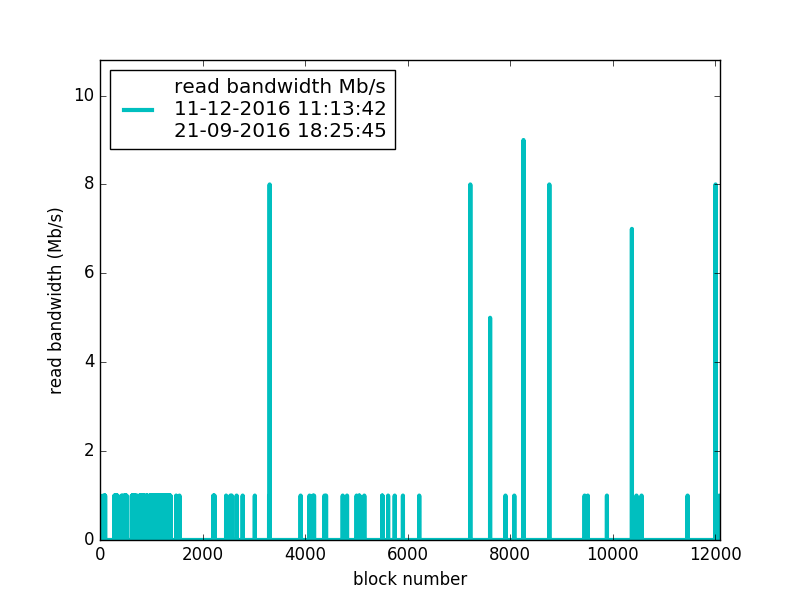
\includegraphics[width=0.9\textwidth]{img/bandwidth}
%	\caption{Read bandwidth of the Bitcoin blockchain measured according to
%		the size of the block fetched and the time taken to fetch that block.
%		Measurement done Measurement done from $21^{st}$~September~$2016$ until
%		$11^{th}$~December~$2016$.}
%	\label{fig:bandwidth}
%\end{figure}

%In Figure~\ref{fig:comparison_visibility_blockcreation} is represented the comparison between
%the block creation time, Figure~\ref{fig:time_per_block}, the average visibility time for
%transactions in each block,
%Figure~\ref{fig:transaction_visibility}, and the the transaction
%visibility provided from the Bitcoin website, Figure~\ref{fig:transaction_visibility_bitcoinwebsite}.
%The comparison was made using exactly the same
%blocks, retrieved from $4^{th}$ until $12^{th}$~December~$2016$. The first thing to notice is that,
%despite the block creation time is never higher than $80$\,minutes, is that there are some
%transactions
%that take more than $1$\,day to be visible. This because miners gives the priority to transactions that are
%willing to pay an higher fee. A lot of transactions are not paying any fee, so they
%will not be included immediately to the next block creation. This thing was not very well explained anywhere
%and it was clear only after this data analysis.
%
%The plot from \url{blockchain.info} in Figure~\ref{fig:transaction_visibility_bitcoinwebsite} shows that,
%in one month, the average confirmation time is~$\sim10$\,minutes, with a peak of $16$.
%Considering though a finer granularity, in about a week of transactions, as shows Figure~\ref{fig:transaction_visibility},
%there is yes a coarse median of~$\sim10$-$20$ minutes, but there are a lot $40$ minutes peaks, some peaks
%of $300$ and $400$ minutes and even others of $1000$ and $1900$ minutes.
%This data might be relevant for a big company who decides to invest a lot in Bitcoin, then
%they need to know that a transaction could take even $100x$ time than what is showed
%in the Bitcoin website.
%
%\begin{figure}[H]
%		\centering
%	\begin{subfigure}{.7\textwidth}
%		\centering
%		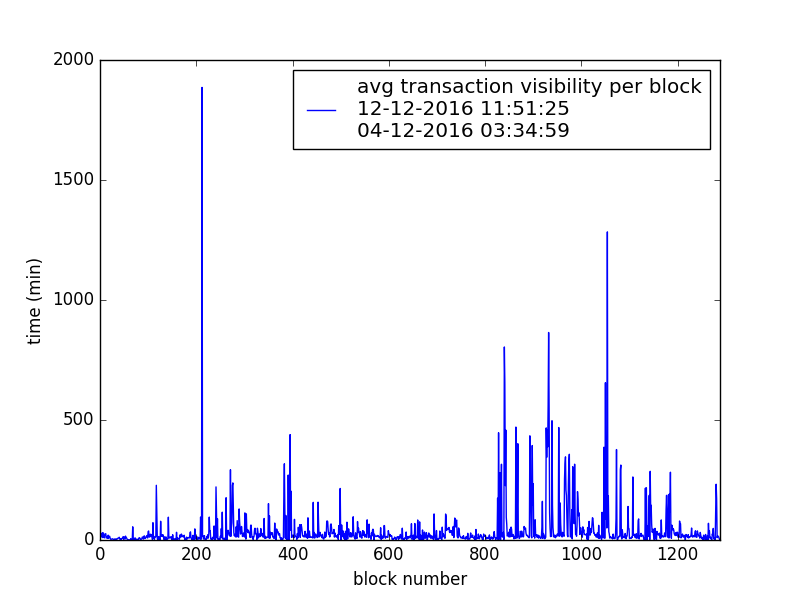
\includegraphics[width=1\linewidth]{img/transaction_visibility}
%		\caption{Average time for a transaction to be visible in the public ledger since
%			its first creation request.
%			Measurement done between $4^{th}$ and $12^{th}$~December~$2016$ on the
%			Bitcoin blockchain.}
%		\label{fig:transaction_visibility}
%	\end{subfigure}%
%
%	\begin{subfigure}{.7\textwidth}
%		\centering
%	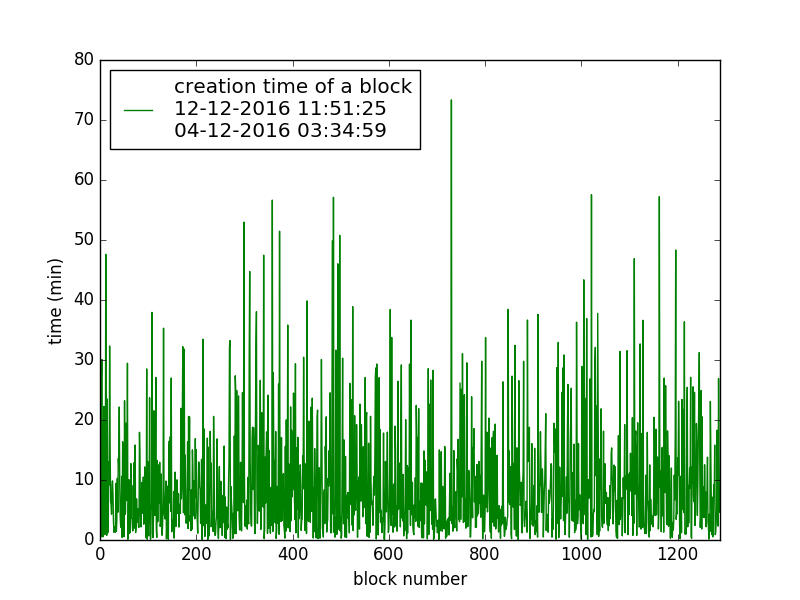
\includegraphics[width=1\textwidth]{img/time_per_block}
%	\caption{The block's creation time in the Bitcoin blockchain. Every block is
%		created each $m$ minutes. Data from $4^{th}$ until $12^{th}$~December~$2016$ are
%		considered for this test.}
%	\label{fig:time_per_block}
%	\end{subfigure}
%	
%	\begin{subfigure}{.7\textwidth}
%			\centering
%		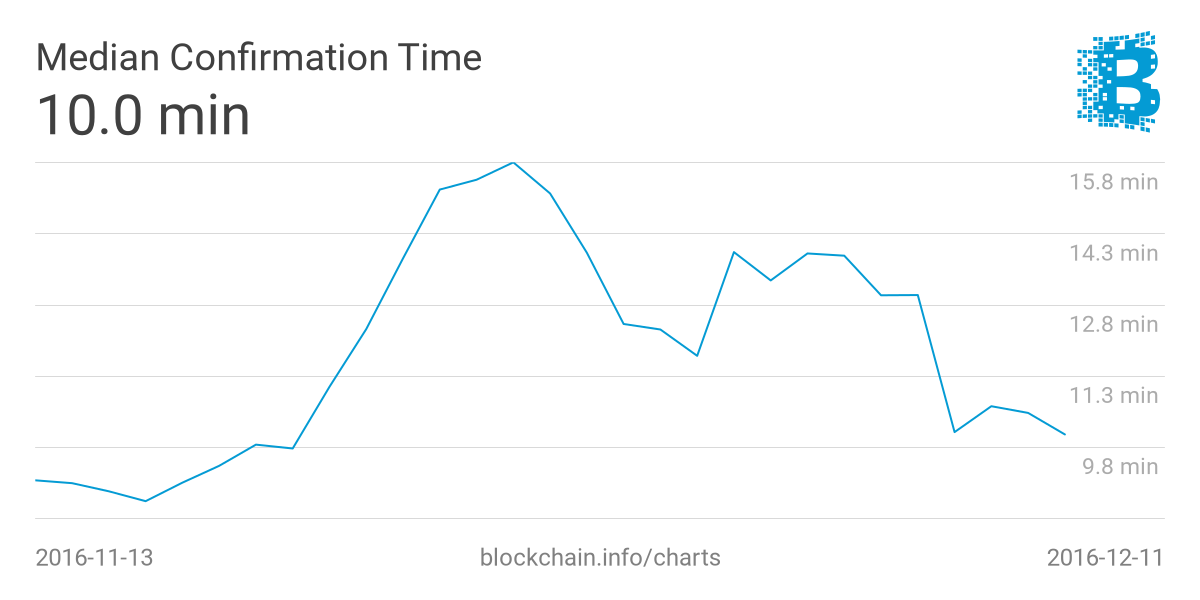
\includegraphics[width=1\textwidth]{img/transaction_visibility_bitcoinwebsite}
%		\caption{Median confirmation time for a transaction. Data from the official Bitcoin website
%			\url{blockchain.info} \cite{bitcoin_blockchain}.}
%		\label{fig:transaction_visibility_bitcoinwebsite}
%	\end{subfigure}
%	\caption{Comparison between block size and the average time for a transaction to be visible in the public ledger.}
%	\label{fig:comparison_visibility_blockcreation}
%\end{figure}

\section{Block Fee}
\label{sec:block-fee}
%In this thesis we aim to find a relation between
%the fee paid to the miner and the block creation time. Before, we saw
%that more a client is willing to pay for a transaction fee ($T_g$) more are
%the probability that its transaction is included immediately in the next block.
%Here we want to confirm the relation that exists between the creation time
%and the fee paid to the miner. In Figure~\ref{fig:fee_bandwidth} an analysis
%between the $21^{st}$~September~$2016$ and the $12^{th}$~December~$2016$
%is done, retrieving $12100$ blocks, and it is pretty clear that there is a certain
%relation between the series of data analyzed. This confirms that,
%more computational effort is put into a block creation and more fee
%is paid to the miner or pool of miners who solve the proof of work.
%Of course there are occasional exceptions, if a block contains a lot of transaction
%with $T_g$ equal to zero, the fee paid to the miner will be lower if compared to
%the one given from a block containing only high priority transactions, which is extremely unfair.
%This is why current, decentralized digital currencies are trying to avoid transactions
%with $T_g$ equal to zero by ignoring them. On the other hand the Figure~\ref{fig:fee_bandwidth}
%shows that there are only couple of blocks that take high computational time, $\sim35$-$38$\,minutes, and get
%a low reward, almost $0$\,\gls{btc}.
%\begin{figure}[H]
%	\centering
%	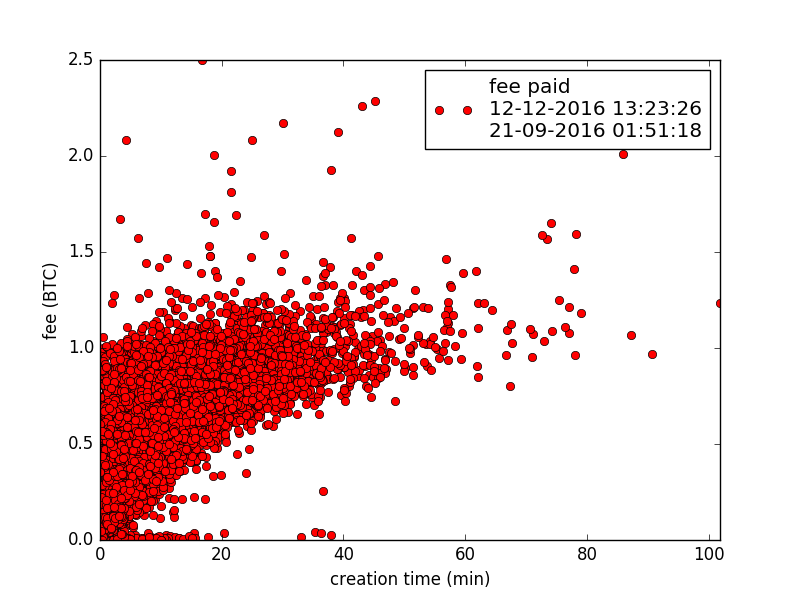
\includegraphics[width=1\textwidth]{img/fee_bandwidth}
%	\caption{Relation between the fee paid to the miner and the block creation time.
%		Measurement done on the Bitcoin blockchain between
%		the $21^{st}$~September~$2016$ and the $12^{th}$~December~$2016$.}
%	\label{fig:fee_bandwidth}
%\end{figure}
%With this observation, it becomes possible to generate a model that,
%in future implementation, could help blocks to get the expected reward for mining. The model
%created is showed in Chapter~\ref{sec:models} and it is generated with the
%polynomial interpolation of the data in Figure~\ref{fig:fee_bandwidth}.

\section{Models}
\label{sec:models}

%Next, we generate a model
%that predict the future growth of the blockchain and help nodes to smartly use their bandwidth.
%To get the model for the blockchain growth, data are collected and then a statistical
%regression is made on them. The function that represents the blockchain growth is obtained
%thanks to the \emph{NumPy} libraries\,\cite{scipy}. To find the model that more fits our data, polynomial
%interpolation was applied\,\cite{Hildebrand:1987:INA}. An example of the code regarding it is found
%in Appendix~\ref{lst:polynomial-interpolation}.

%\begin{figure}[H]
%	\centering
%	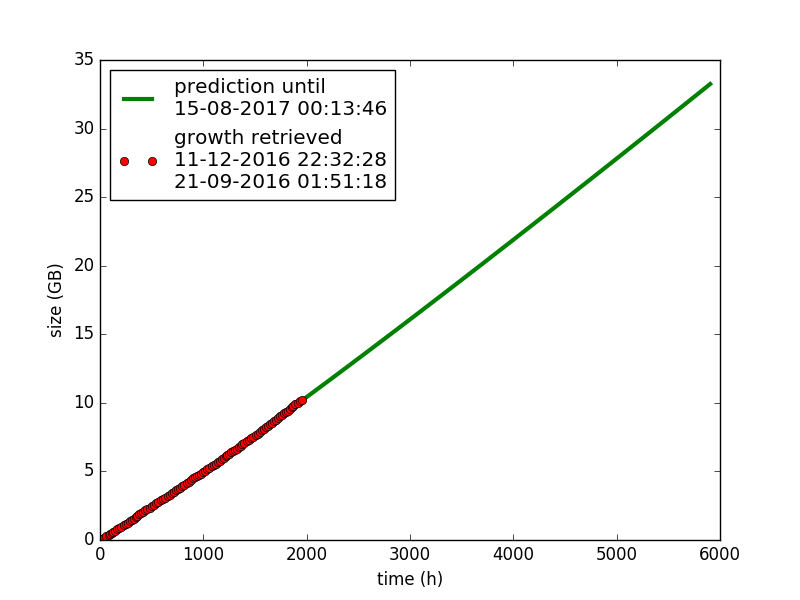
\includegraphics[width=1\textwidth]{img/regression_growth_blockchain}
%	\caption{Regression of the growth of the blockchain with a prediction model.
%		Measurement done on the
%		Bitcoin blockchain between the $21^{st}$~September~$2016$ and the
%		$11^{th}$~December~$2016$.}
%	\label{fig:regression_growth}
%\end{figure}

%Considering the blockchain growth, a prediction of $3x$ time in the future has been evaluated. If
%the evaluation is done considering $1000$\,blocks, with a total time of $150$\,hours, then the
%prediction will be on how much the blockchain will grow in the following $300$\,hours.
%The Figure~\ref{fig:regression_growth} shows that the blockchain, as expected, has an
%almost linear growth. It has though a very little quadratic coefficient due to the
%slightly increment of the block size among the years. The function evaluated using the polynomial
%interpolation for the blockchain growth is the following:
%\begin{equation}
%\label{eq:growth_regression}
%f_g(x) = \frac{9}{10^8}x^2 + \frac{5}{10^{3}}x
%\end{equation}
%According to the prediction in Figure~\ref{fig:regression_growth}, analyzing data
%from $21^{st}$~September until $11^{th}$~December~$2016$, the blockchain
%will grow of $\sim28$\,GB by August~$2017$.
%To verify the veracity of this prediction, we applied this method from September~$2016$
%to December~$2016$ so that we have the real growth to compare. Even though the data
%used were not so many ($2000$ blocks for $1$ month forecast compared to the $12200$\,blocks
%used in the Figure~\ref{fig:regression_growth}), they were accurate in the prediction.
%That model has told us that by the $14^{th}$ of December~$2016$ the blockchain was
%supposed to grow of $9,5$\,GB, when only data from September~$2016$
%were evaluated. The blockchain has grown with about $10$\,GB instead, but
%still, considering the few data analyzed, the model generated is accurate and reliable.
%More data are used for the prediction, more accurate will be the function generated.
%
%\begin{figure}[h]
%	\centering
%	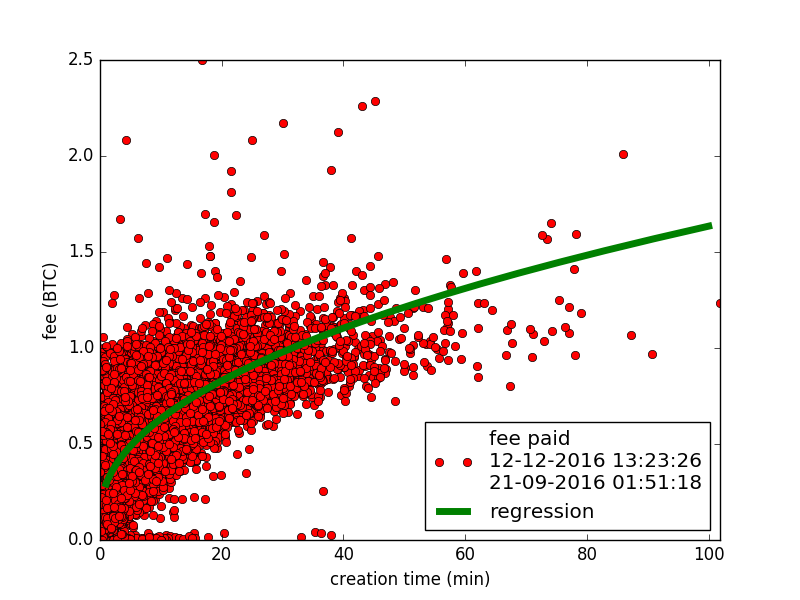
\includegraphics[width=1\textwidth]{img/fee_regression}
%	\caption{Regression of the relation between the fee paid
%		to the miner and the block creation time.
%		Measurement on the Bitcoin blockchain between
%		the $21^{st}$~September~$2016$ and
%		the $12^{th}$~December~$2016$.}
%	\label{fig:fee_regression}
%\end{figure}

%The Figure~\ref{fig:fee_regression} shows that there is a relation between the fee paid
%and the creation time of a block. This relation seems to be quadratic/logarithmic.
%The regression is found using NumPy libraries~\cite{scipy} and the function is obtained
%with the polynomial interpolation. More data are analyzed, more the function
%generated is accurate. The one showed below in (\ref{eq:fee_regression}) is created
%by collecting data from  $21^{st}$~September~$2016$ until $12^{th}$~December~$2016$. 
%\begin{equation}
%\label{eq:fee_regression}
%f_{Bg}(x) =  \begin{cases}-\frac{1}{10^4}x^2 + \frac{3}{10^2}x + 0,3 & \mbox{ with } x < 100 \end{cases}
%\end{equation}
%Note that this function is valid if the creation time, $x$, is
%lower than $100$\,minutes.
%This model could be useful for a miner which expects a certain fee after mining for \emph{n}
%minutes, to see if the fee they received is below or above the function model. In that way for the next
%mining processes a block will be in debit or credit and he will consider only transaction with an higher
%$T_g$, or transaction with a lower $T_g$ according of how much is its credit/debit.
%
%The last model generated is showed in Figure~\ref{fig:transaction_fee_bandwidth}. It
%represents the average approval time for the transactions in a block, compared to
%the fee paid ($B_g$) divided by the number of transactions in that particular block.
%Then for each block $B$ we calculated the average $T_p$, $\overline{T_p}$, as:
%\begin{equation}
%\label{eq:transaction_fee}
%\overline{T_p} = \frac{B_g}{|B_t|} 
%\end{equation}
%where $|B_t|$ is the number of transactions approved from the block $B$.
%The plot in Figure~\ref{fig:transaction_fee_bandwidth} shows that if a transaction
%pays from $0$ to $0.001$\,\gls{btc}, then the visibility would be almost random.
%However if their $T_g$ is increased from $0.002$ and $0.006$\,\gls{btc} their
%visibility will be seldom above $35$\,minutes and most likely between $5$ and $15$\,minutes.
%The function generated with the polynomial interpolation is the following:
%\begin{equation}
%\label{eq:transaction_fee_bandwidth}
%f_t(x) = \begin{cases}\frac{1}{10^8}x^2 - 5000x + 35 & \mbox{ with } x < 0.007\end{cases}
%\end{equation}
%The function showed in~(\ref{eq:transaction_fee_bandwidth}) is important
%for a transaction that needs a certain bandwidth, in a way that it knows, approximately, how much
%$T_g$ should be willing to pay according to get a positive bandwidth.
%
%\begin{figure}[h]
%	\centering
%	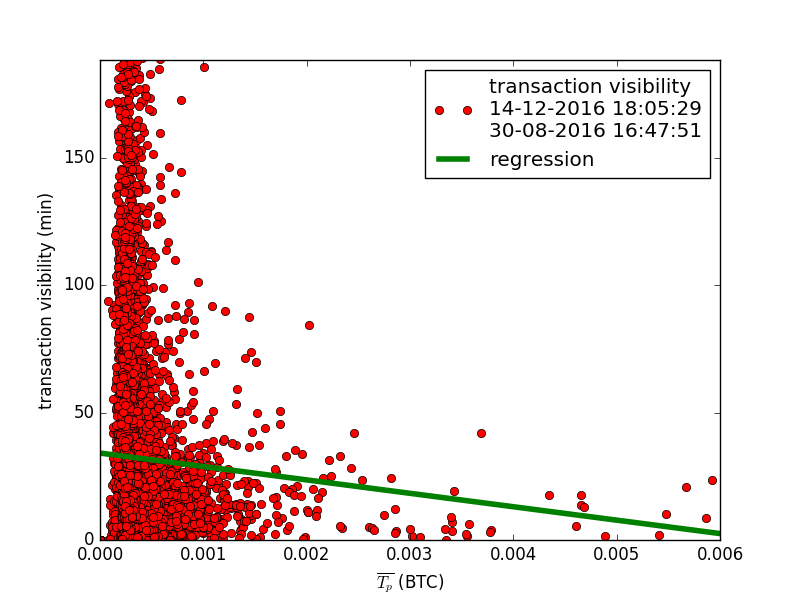
\includegraphics[width=1\textwidth]{img/transaction_fee_bandwidth}
%	\caption{Regression of the relation between the fee paid
%		to the miner and the transaction visibility time.
%		Measurement on the Bitcoin blockchain between
%		the $30^{th}$\,August $2016$ and the
%		$14^{th}$\,December $2016$.}
%	\label{fig:transaction_fee_bandwidth}
%\end{figure}

\chapter{Conclusions}
\label{chap:conclusion}
%This chapter talks about the future implementation of the analytics system, what are
%the most relevant data to analyze in the future and how they could be implemented
%and evaluated.
%These considerations are made after profiling the system. The chapter discusses also
%about the model generated,  showed
%in Chapter~\ref{sec:models}, their accuracy and their reliability.
%In Chapter~\ref{sec:future_implementation}, we 
%show how the system could change following some design pattern solution.

\section{Discussion}
\label{sec:discussion}
%We are satisfied about the models generated, showed in Chapter~\ref{sec:models}.
%The blockchain growth prediction turned out to be accurate even with couple
%of months of analysis, and the more data are collected the more precise it will be.
%Since when the first block was appended, in $2009$, the block size kept increasing. Even if this
%size changed only from $200$\,kB to $1$\,MB, it is still enough to have a quadratic growth from
%$2009$ until $2016$, while Bitcoin said it would have been linear.
%
%Despite that we found a relation between the fee and the block creation time, the
%creation of a block is still a random process, determined from the proof of work, and paying
%so much fee ($T_g$) will not guarantee an extremely fast execution. Of course your
%transaction will be considered as "high priority" and included in the block that is being
%mined at the moment, but still the bandwidth is limited from the mining difficulty, the random process
%of hash generation and from the computational power of the miners. However, thanks to the plot
%showed in Figure~\ref{fig:transaction_fee_bandwidth} we can conclude that if the $T_g$ of a single
%transaction is higher than $0.003$\,\gls{btc}, then its visibility in the ledger of data will not be
%more that $50$\,minutes.

\section{Future Implementation}
\label{sec:future_implementation}
%Before of thinking about the future implementation, an analysis on the
%current system has to be done. The blockchain analytics system was evaluated using a line profiler for
%Python\,\cite{line_profiler}. The results, showed in Figure~\ref{fig:profile}, are that the biggest
%computation in matter of time is the retrieval of the blocks.
%The \gls{api} calls with blockexplorer methods take indeed $\sim98\%$ of the time retrieving
%$500$ blocks, while the writing part and the plotting part together take $\sim1.4\%$
%of the total time. This is why the fetching and the analysis part are now separated.
%This separation will allow in the future to analyze a bigger portion of the blockchain,
%to manipulate more data and to get much more information from it.
%This also allows to do the analysis in a much faster way, from $17,5$\,minutes,
%fetching $500$ blocks, it could take only $\sim2$\,seconds if
%the file containing the blockchain is already generated.

%\begin{figure}[h]
%	\centering
%	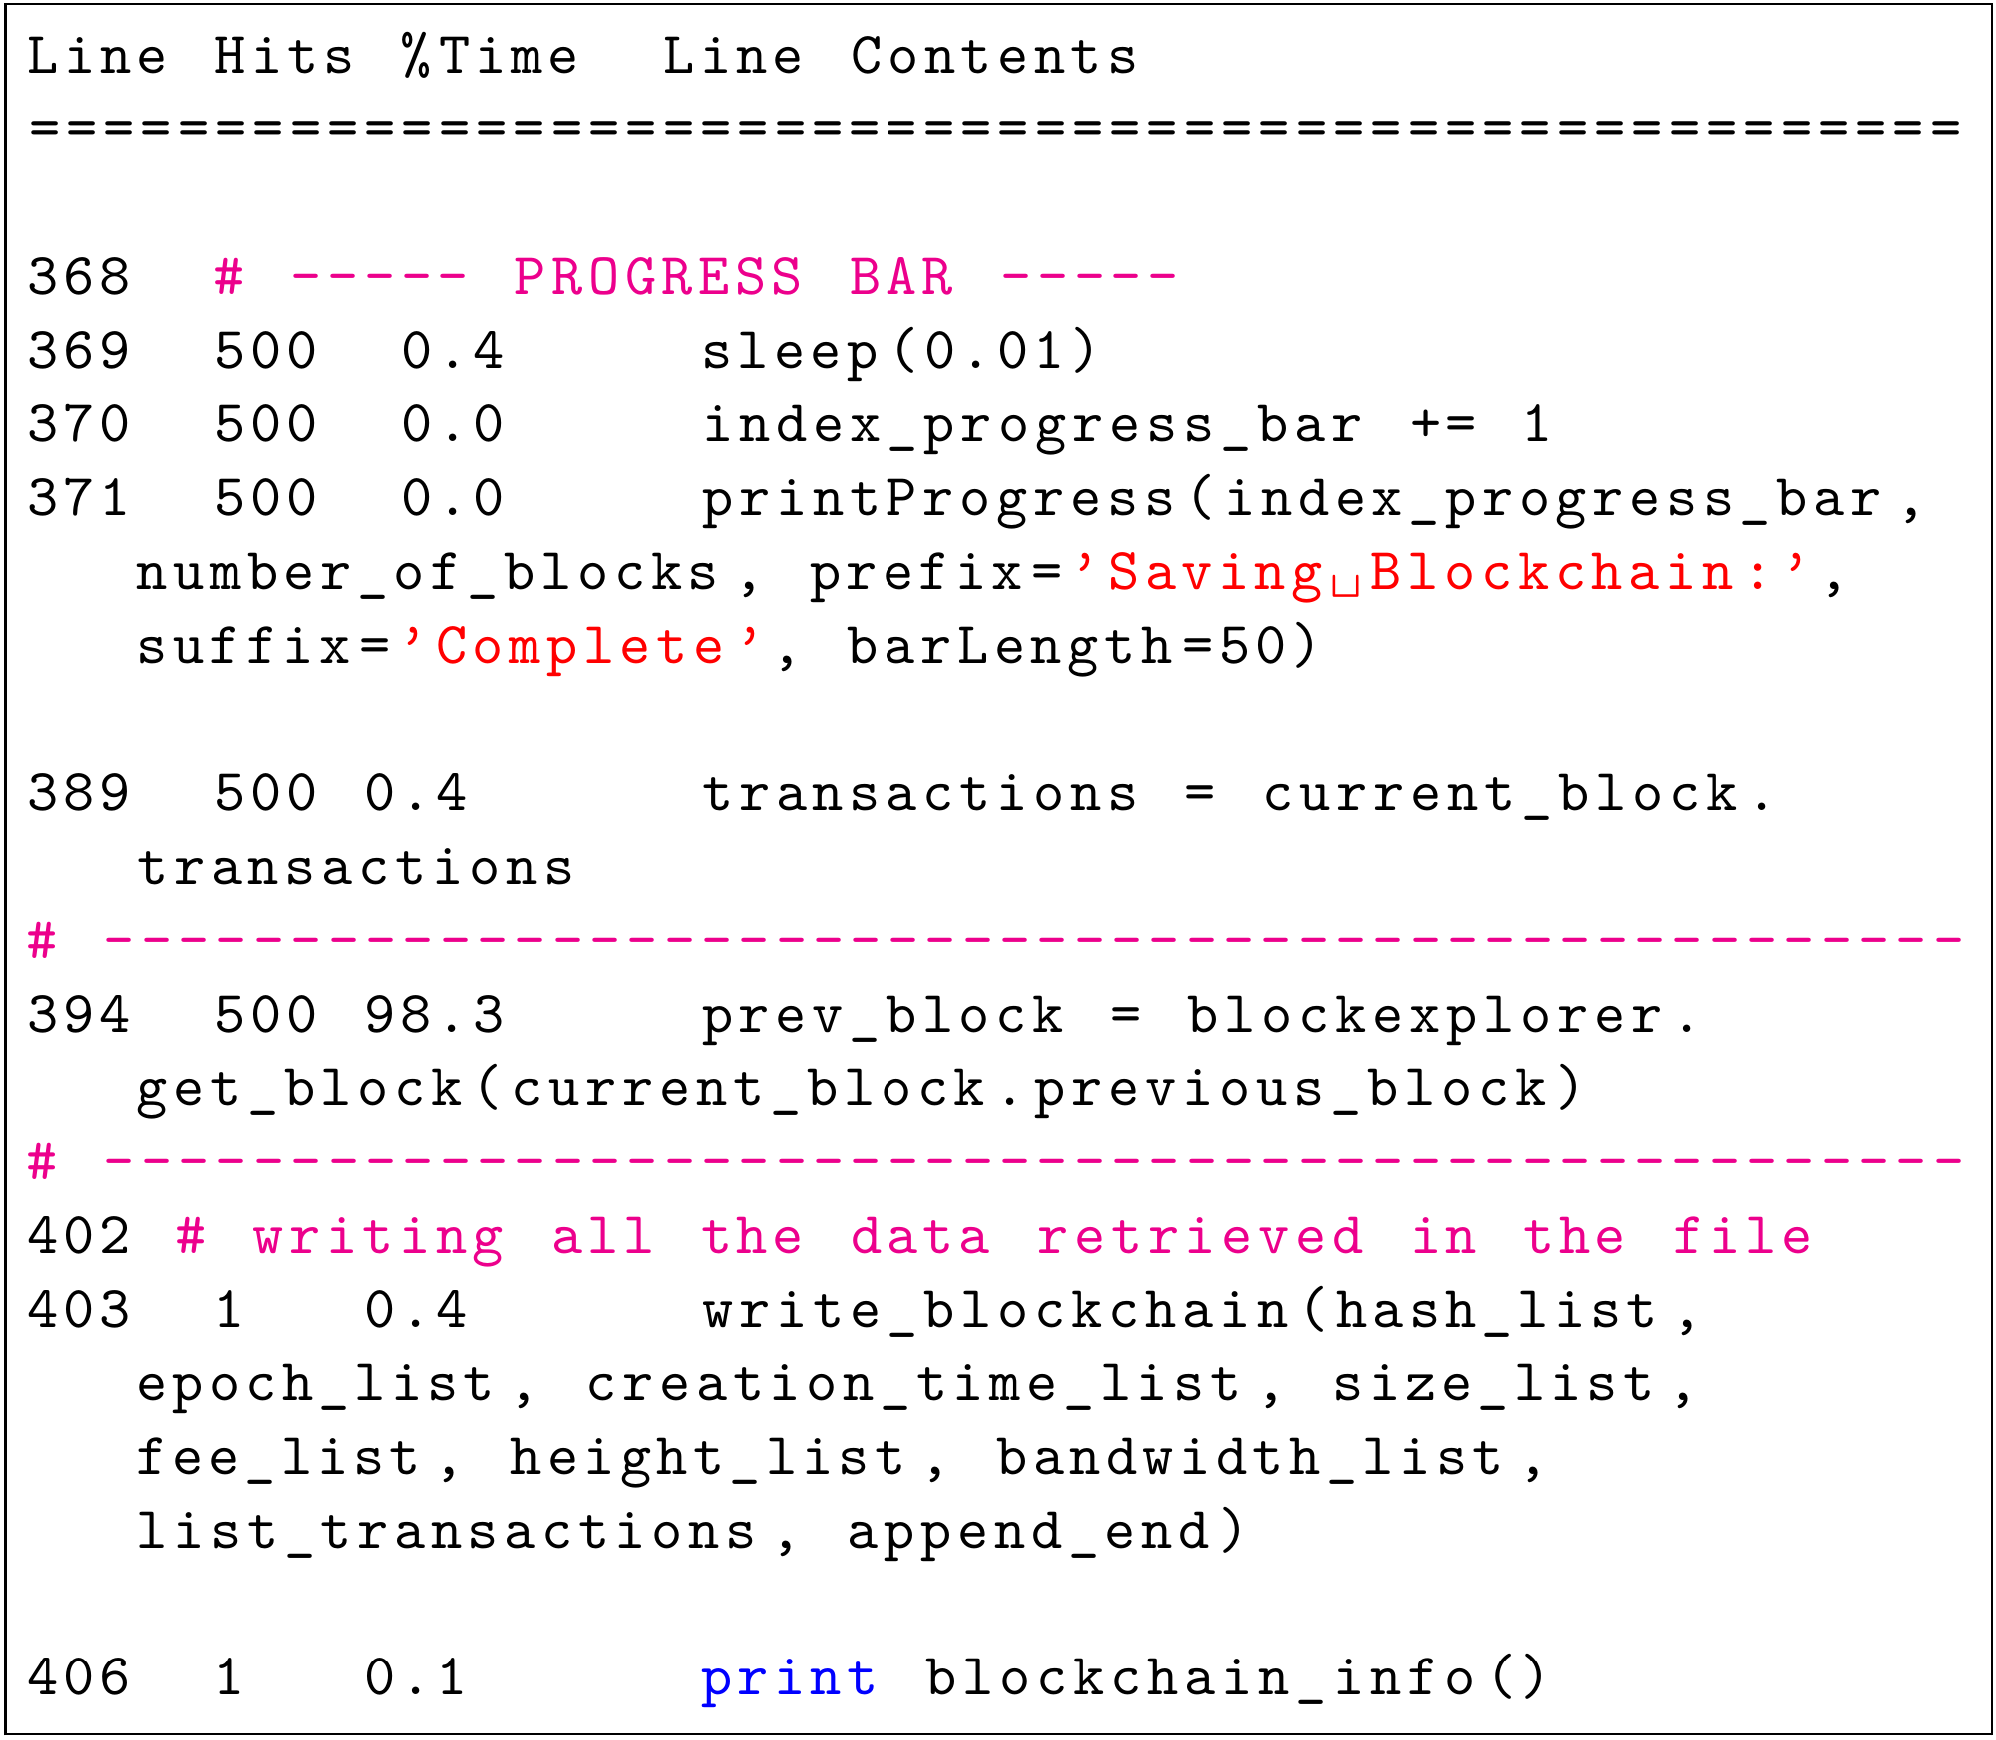
\includegraphics[width=1\textwidth]{img/profile}
%	\caption{Profiling results while executing the system retrieving $500$ blocks}
%	\label{fig:profile}
%\end{figure}
%
%In future implementation more data from each block could be considered, such
%as the correctness of every block created. Correctness for each block is a value obtained
%putting all the most important informations of a block in a multidimensional vector, in the
%following way:
%\begin{equation}
%\label{eq:correctness_vector}
%	C=\begin{bmatrix}
%		B_{sz} \\
%		B_g\\
%		B_s\\
%		B_t
%	\end{bmatrix}
%\end{equation}
%considering for each block the size ($B_{sz}$), the fee ($B_g$), the epoch,
%transformed in creation time ($B_s$) and the
%number of transactions in this block ($B_t$).
%The correctness of a block then is dependent from the range of these values
%and this range can change according to the level of correctness desired.
%For example we could have:
%\begin{equation}
%C_B = \begin{cases}
%300 < B_{sz} \leqslant 1000, & \mbox{bytes} \\
%0.5 < B_g < 1.5, & \mbox{BTC} \\
%6 < B_s < 12, & \mbox{minutes} \\
%500 < B_t < 1500, & \mbox{transactions}
%\end{cases}
%\end{equation}
%Which means that a block is correct if the correctness for this block, $C_B$, respects
%these values. In that way is possible to calculate how many blocks among the
%retrieved ones can be considered correct. It will be also possible to add the percentage
%of each correct/incorrect field, to find any possible relation between those and to get
%information about whether a block is incorrect, why that happened.
%It is already implemented, but not tested yet, the relation between the average
%transaction time and the fee paid to mine a block.
%Furthermore, following the design pattern principles, refactoring on the code must be done since
%the method \emph{write\_blockchain()} contains some \emph{duplicate code} about writing on
%the file. The treatment to use might be \emph{extract method} on the \emph{file.write}.

\section{Comments}
\label{sec:comments}
%A relevant aspect to note is that there are some blocks
%that take approximately $80$\,minutes to be created, when the
%average time is supposed to be $\sim8$\,min. This affects also the
%transaction visibility but it is also a side effect of the difficulty
%and proof of work. Furthermore, the growth of the blockchain
%is not $\sim1$\,MB per hour as claimed from Bitcoin in $2008$
%but, at the moment, $\sim5$\,MB each hour, growing of $\sim2$\,GB in less than $12$\,days.
%In conclusion, we demonstrate our thesis and found a relation between the fee paid to a miner
%and the block creation time. We generate a function which describes this relation and it can
%be used in future implementations, allowing miners to be fairly rewarded.
%A block can arbitrary decides whether ignore a transaction
%that is not willing to pay enough fee ($T_g$).
%Plus, we defined a model for growth prediction and we tested its accuracy. Finally, a portion of
%the blockchain is saved locally and more analysis on it are possible in the future.

show bibliography \cite{Nakamoto_bitcoin}, \cite{ethereum}, \cite{Back02hashcash},
\cite{Dwork:1992}, \cite{Luu:2016}, \cite{Delmolino2016},
\cite{ethereum_white_paper}, \cite{ethereum_solidity}, \cite{Luu:2015:DIC},
\cite{sha}, \cite{Hopcroft:2006:IAT}, \cite{Johansen2015Fireflies}, \cite{bitcoinmining},
\cite{Garcia:2011:EMB}, \cite{vandiver2007hrdb},
\cite{Luiz:2014:MBF}, \cite{bitcoin_api}, \cite{ethereum_api}, \cite{merkle_tree}, \cite{ethereum_wiki_patricia_tree},
\cite{swan2015blockchain}, \cite{Baran1964:ODC}, \cite{Stallings:2002:CNS}, \cite{bitcoin_blockchain}, \cite{ethereum_bc_analysis},
\cite{ethereum_blockchain}, \cite{bitcoinmining_process},
\cite{tradeblock}, \cite{ethereum_website}, \cite{Larman:2004:AUP},
\cite{Aho:1992:FCS}, \cite{matplotlib}, \cite{croman2016}, \cite{DBLP:journals/corr/EyalGSR15},
\cite{Hildebrand:1987:INA}, \cite{mining_hw}, \cite{hashing_rate}, \cite{bitnodes}, \cite{Rizun:2015:blocksizelimit}
\cite{linearize}, \cite{Tedeschi:2016:PBB}.


\bibliographystyle{plain}
\bibliography{thesis}

\begin{appendices}
	\chapter{Terminology}
	\label{app:terminology}
	\begin{description}
		\item[RLP:] Stands for recursive length prefix. It is a serialization method
		for encoding arbitrary structured binary data (byte arrays).
		\label{item:rlp}
		\item[KEC-256:] Another serialization method generating a 256-bit hash.
		\item[full node:] A full node in a decentralized digital currency peer-2-peer network, is a node that stores
		and processes the entirety of every block, storing locally the entire size of the blockchain.
		\item[light node:] A light node in a decentralized digital currency peer-2-peer network, is a node that only
		stores the part of the blockchain it needs.
		\item[satoshi:] Unit of the Bitcoin currency. 100,000,000 satoshi are 1 BTC (Bitcoin).
	\end{description}
	\chapter{Listing}
	\label{app:listing}
	\begin{lstlisting}[numbers=left,frame=single,caption={Smart contract transaction code in Ethereum.}]
function transfer(address _to, uint256 _value) {
	/* Add and subtract new balances */
	balanceOf[msg.sender] -= _value;
	balanceOf[_to] += _value;
	}
	\end{lstlisting}
	
	\lstset{language=Python,
	basicstyle=\ttfamily,
	keywordstyle=\color{blue}\ttfamily,
	stringstyle=\color{red}\ttfamily,
	commentstyle=\color{green}\ttfamily,
	breaklines=true,
	morecomment=[l][\color{magenta}]{\#},
	label = {lst:smartcontract}
}
\begin{lstlisting}[float, numbers=left,frame=single,caption={Example of a smart contract that rewards users who solve a computational puzzle~\cite{smartcontracts}.}]
contract Puzzle {
  address public owner ;
  bool public locked ;
  uint public reward ;
  bytes32 public diff ;
  bytes public solution ;

  function Puzzle () // constructor {
    owner = msg. sender ;
    reward = msg . value ;
    locked = false ;
    diff = bytes32 (11111); // pre - defined difficulty
    }

  function (){ // main code , runs at every invocation
    if ( msg. sender == owner ){ // update reward
    if ( locked )
    throw ;
    owner . send ( reward );
    reward = msg . value ;
    }
    else
      if ( msg . data . length > 0){ // submit a solution
      if ( locked ) throw ;
      if ( sha256 (msg. data ) < diff ){
          msg. sender . send ( reward ); // send reward
          solution = msg. data ;
          locked
          }}}}
\end{lstlisting}

	\lstset{language=Python,
	basicstyle=\ttfamily,
	keywordstyle=\color{blue}\ttfamily,
	stringstyle=\color{red}\ttfamily,
	commentstyle=\color{green}\ttfamily,
	breaklines=true,
	morecomment=[l][\color{magenta}]{\#},
	label = {lst:usage}
}
\begin{lstlisting}[float, numbers=left, frame=single, caption={Application usage.}]
Usage: observ.py -t number
  -h | --help    : usage
  -i             : gives info of the blockchain in the file .txt
  -t number      : add on top a number of blocks. The blocks retreived will be the most recent ones. If the blockchain growth more than the block requested do -u (update)
  -e number      : append blocks at the end of the .txt file. Fetch older blocks starting from the last retrieved
  -P             : plot all
  -p start [end] : plot data in .txt file in a certain period of time, from start to end. If only start then consider from start to the end of the .txt file
  -R             : plot the regression and the models that predict the blockchain
  -r start [end] : plot the regression and the models in a certain period of time, from start to end. If only start then consider from start to the end of the .txt file
  -u             : update the local blockchain to the last block created

\end{lstlisting}


	\lstset{language=Python,
	basicstyle=\ttfamily,
	keywordstyle=\color{blue}\ttfamily,
	stringstyle=\color{red}\ttfamily,
	commentstyle=\color{green}\ttfamily,
	breaklines=true,
	morecomment=[l][\color{magenta}]{\#},
	label = {lst:block}
}

\begin{lstlisting}[float, numbers=left,frame=single,caption={Block object represented in Python according to api-v1-client-python to retrieve data on the blockchain. The function get\_block() will return an object of this type\,\cite{bitcoin_api}.},language=Python]
class Block:
  def __init__(self, b):
    self.hash = b['hash']
    self.version = b['ver']
    self.previous_block = b['prev_block']
    self.merkle_root = b['mrkl_root']
    self.time = b['time']
    self.bits = b['bits']
    self.fee = b['fee']
    self.nonce = b['nonce']
    self.n_tx = b['n_tx']
    self.size = b['size']
    self.block_index = b['block_index']
    self.main_chain = b['main_chain']
    self.height = b['height']
    self.received_time = b.get('received_time', b['time'])
    self.relayed_by = b.get('relayed_by')
    self.transactions = [Transaction(t) for t in b['tx']]
    for tx in self.transactions:
        tx.block_height = self.height
\end{lstlisting}

	\lstset{language=Python,
	basicstyle=\ttfamily,
	keywordstyle=\color{blue}\ttfamily,
	stringstyle=\color{red}\ttfamily,
	commentstyle=\color{green}\ttfamily,
	breaklines=true,
	morecomment=[l][\color{magenta}]{\#},
	label = {lst:transaction}
}

\begin{lstlisting}[float, numbers=left,frame=single,caption={Transaction object represented in Python according to api-v1-client-python to retrieve data on the blockchain. The function get\_transaction() will return an object of this type\,\cite{bitcoin_api}.},language=Python]
class Transaction:
  def __init__(self, t):
    self.double_spend = t.get('double_spend', False)
    self.block_height = t.get('block_height')
    self.time = t['time']
    self.relayed_by = t['relayed_by']
    self.hash = t['hash']
    self.tx_index = t['tx_index']
    self.version = t['ver']
    self.size = t['size']
    self.inputs = [Input(i) for i in t['inputs']]
    self.outputs = [Output(o) for o in t['out']]

    if self.block_height is None:
       self.block_height = -1
\end{lstlisting}

	\lstset{language=Python,
	basicstyle=\ttfamily,
	keywordstyle=\color{blue}\ttfamily,
	stringstyle=\color{red}\ttfamily,
	commentstyle=\color{green}\ttfamily,
	breaklines=true,
	morecomment=[l][\color{magenta}]{\#},
	label = {lst:block-json}
}

\begin{lstlisting}[float, frame=single, caption={Json object returned from the method \emph{get\_block()} in the Bitcoin \gls{api} class blockexplorer.py\,\cite{bitcoin_api}}, language=Python]
hash : str
version : int
previous_block : str
merkle_root : str
time : int
bits : int
fee : int
nonce int
n_tx : int
size : int
block_index : int
main_chain : bool
height : int
received_time : int
relayed_by : string
transactions : array of Transaction objects
\end{lstlisting}


	\lstset{language=Python,
	basicstyle=\ttfamily,
	keywordstyle=\color{blue}\ttfamily,
	stringstyle=\color{red}\ttfamily,
	commentstyle=\color{green}\ttfamily,
	breaklines=true,
	morecomment=[l][\color{magenta}]{\#},
	label = {lst:latest-block}
}
\begin{lstlisting}[float, numbers=left,frame=single,caption={Structure of the latest block retrieved. The function get\_latest\_block() will return an object with this structure.}]
class LatestBlock:
def __init__(self, b):
self.hash = b['hash']
self.time = b['time']
self.block_index = b['block_index']
self.height = b['height']
self.tx_indexes = [i for i in b['txIndexes']]
\end{lstlisting}


\lstset{language=Python,
	basicstyle=\ttfamily,
	keywordstyle=\color{blue}\ttfamily,
	stringstyle=\color{red}\ttfamily,
	commentstyle=\color{green}\ttfamily,
	breaklines=true,
	morecomment=[l][\color{magenta}]{\#},
	label = {lst:append-block}
}
\begin{lstlisting}[float, numbers=left, frame=single, caption={Collecting data starting from the last element in the blockchain.txt file.}]
earliest_hash = get_earliest_hash()
get_blockchain(n, earliest_hash)

def get_blockchain(n, hash = None):
  [...]
  if (hash):  # start the retrieval from the hash
    append_end = True  # in that way the write_blockchain method knows that has to append blocks and not write them at the beginning
    last_block = blockexplorer.get_block(hash)
  [...]

def get_earliest_hash():
  hash_list = get_list_from_file("hash") # method to collect data from blockchain.txt file having as attribute "hash"
  length = len(hash_list)
  earliest_hash = hash_list[length - 1]
  return earliest_hash
\end{lstlisting}


	\lstset{language=Python,
	basicstyle=\ttfamily,
	keywordstyle=\color{blue}\ttfamily,
	stringstyle=\color{red}\ttfamily,
	commentstyle=\color{green}\ttfamily,
	breaklines=true,
	morecomment=[l][\color{magenta}]{\#},
	label = {lst:api-python}
}
\begin{lstlisting}[float, numbers=left, frame=single,caption={Calling \url{blockchain.info} through python \gls{api} and retrieving part of the blockchain.}]
from blockchain import blockexplorer
# get the last block
last_block = blockexplorer.get_latest_block()
hash_last_block = last_block.hash

# current block now is the last block
current_block = blockexplorer.get_block(hash_last_block)
\end{lstlisting}

	\lstset{language=Python,
	basicstyle=\ttfamily,
	keywordstyle=\color{blue}\ttfamily,
	stringstyle=\color{red}\ttfamily,
	commentstyle=\color{green}\ttfamily,
	breaklines=true,
	morecomment=[l][\color{magenta}]{\#},
	label = {lst:read-bandwidth},
	numbers=left,
	frame=single
}
\begin{lstlisting}[float, caption={How read bandwidth is calculated, using the function $datetime.now()$ before and after the \gls{api} call.}]
start_time = datetime.datetime.now() # ---------
current_block = blockexplorer.get_block(current_block.previous_block)
end_time = datetime.datetime.now() # ---------
time_to_fetch = end_time - start_time
time_in_seconds = get_time_in_seconds(time_to_fetch)

#latency
fetch_time_list.append(time_in_seconds)

# calculate Bandwidth with MB/s
block_size = float(current_block.size) / 1000000
bandwidth = block_size / time_in_seconds
bandwidth_list.append(bandwidth)
\end{lstlisting}

	\lstset{language=Python,
	basicstyle=\ttfamily,
	keywordstyle=\color{blue}\ttfamily,
	stringstyle=\color{red}\ttfamily,
	commentstyle=\color{green}\ttfamily,
	breaklines=true,
	morecomment=[l][\color{magenta}]{\#},
	label = {lst:get-transaction-time},
	numbers=left,
	frame=single
}
\begin{lstlisting}[float, caption={Function that get the average write bandwidth of the block, calculating the time for each transaction to be visible in the public ledger of data.}]
def get_avg_transaction_time(block):
  # take transactions the block
  transactions = block.transactions

  # get block time -- when it is visible in the blockchain, so when it was created
  block_time = block.time

  # list of the creation time for all the transaction in the block
  transactions_time_list = []

  # list of the time that each transaction needs before being visible in the blockchain
  time_to_be_visible = []

  for t in transactions:
    transactions_time_list.append(float(t.time))

  for t_time in transactions_time_list:
    time_to_be_visible.append(float(block_time - t_time))
    
  average_per_block = sum(time_to_be_visible) / len(time_to_be_visible)
  return average_per_block
\end{lstlisting}

	\lstset{language=Python,
	basicstyle=\ttfamily,
	keywordstyle=\color{blue}\ttfamily,
	stringstyle=\color{red}\ttfamily,
	commentstyle=\color{green}\ttfamily,
	breaklines=true,
	morecomment=[l][\color{magenta}]{\#},
	label = {lst:file-write},
	numbers=left,
	frame=single
}
\begin{lstlisting}[float, caption={How the file.write is performed in the blockchain analytics system. Differences with add and append.}]
if(append):
  for i in range(n):
    file.write("block_informations")

else: # add on top
  hash_list_in_file = get_list_from_file("hash")
  first_hash = hash_list_in_file[0]
  elements = len(hash_list_in_file)
  last_hash = hash_list_in_file[elements-1]
  met_first = False
  with io.FileIO(file_name, "a+") as file:
    file.seek(0)  # place at the beginning of the file
    existing_lines = file.readlines()  # read the already existing lines
    file.seek(0)
    file.truncate()  # delete all the file
    file.seek(0)
    i = 0
    while (i < n):
      if (first_hash == hash[i]):
        met_first = True
      while((met_first == False) and (i < n)):
        # append on top
        file.write("block_informations")
        i = i + 1
        if ((i < n) and (first_hash == hash[i])):
          met_first = True
      # when the block retrieved meets the one alread in the blockchain write the old file
      file.writelines(existing_lines)

\end{lstlisting}

	\lstset{language=Python,
	basicstyle=\ttfamily,
	keywordstyle=\color{blue}\ttfamily,
	stringstyle=\color{red}\ttfamily,
	commentstyle=\color{green}\ttfamily,
	breaklines=true,
	morecomment=[l][\color{magenta}]{\#},
	label = {lst:python-list},
	numbers=left,
	frame=single
}
\begin{lstlisting}[float, caption={Changing all the values inside a Python list in one code line.}]
# size_list from byte to MB
size_list[:] = [x / 1000000 for x in size_list]
# time_list from seconds in minutes
time_list[:] = [x / 60 for x in time_list]
\end{lstlisting}


	\lstset{language=Python,
	basicstyle=\ttfamily,
	keywordstyle=\color{blue}\ttfamily,
	stringstyle=\color{red}\ttfamily,
	commentstyle=\color{green}\ttfamily,
	breaklines=true,
	morecomment=[l][\color{magenta}]{\#},
	label = {lst:get-data-from-file},
	numbers=left,
	frame=single
}
\begin{lstlisting}[float, caption={Method that allows, given an attribute present in the blockchain.txt file, to create a list containing informations only about this quality using \emph{regular expressions}.}]
hash_list = get_list_from_file("hash")

def get_list_from_file(attribute):
  list_to_return = []
  if (os.path.isfile("blockchain.txt")):
    # open the file and read in it -- blockchain_file
    with open("blockchain.txt", "r") as blockchain_file:
      for line in blockchain_file:
      # regular expression that puts in a list the line just read: eg. ['hash', '<block_hash>']
        list = re.findall(r"[\w']+", line)
        # list[0] --> contains the attribute
        # list[1] --> contains the value
        if ((list) and (list[0] == attribute)):
          list_to_return.append(list[1])
  return list_to_return
\end{lstlisting}

	\lstset{language=Python,
	basicstyle=\ttfamily,
	keywordstyle=\color{blue}\ttfamily,
	stringstyle=\color{red}\ttfamily,
	commentstyle=\color{green}\ttfamily,
	breaklines=true,
	morecomment=[l][\color{magenta}]{\#},
	label = {lst:growing-lists},
	numbers=left,
	frame=single
}
\begin{lstlisting}[float, caption={Generation of the growing size and time lists. Calculated following the Equations~\ref{eq:growing_size},~\ref{eq:growing_time}.}]
def create_growing_time_list(time_list):
  reversed_time_list = time_list[::-1]
  time_to_append = 0
  previous_time = 0
  growing_time_list = []
  growing_time_list.append(previous_time)
  for time_el in reversed_time_list:
    time_to_append = (float(time_el) / (60 * 60)) + previous_time  # time in hours
    growing_time_list.append(time_to_append)
    previous_time = time_to_append
  return growing_time_list

def create_growing_size_list(size_list):
  reversed_size_list = size_list[::-1]
  growing_size_list = []
  value_to_append = 0
  size_back = 0
  growing_size_list.append(value_to_append)
  for size_el in reversed_size_list:
    value_to_append = size_el + size_back
    growing_size_list.append(value_to_append)
    size_back = value_to_append
  return growing_size_list
\end{lstlisting}

	\lstset{language=Python,
	basicstyle=\ttfamily,
	keywordstyle=\color{blue}\ttfamily,
	stringstyle=\color{red}\ttfamily,
	commentstyle=\color{green}\ttfamily,
	breaklines=true,
	morecomment=[l][\color{magenta}]{\#},
	label = {lst:polynomial-interpolation},
	numbers=left,
	frame=single
}
\begin{lstlisting}[float, caption={Example of a polynomial interpolation of two lists using NumPy libraries.}]
import numpy as np

model = np.polyfit(list1, list2, deg) # polynomial interpolation between list1 and list2 with the degree of the return polynomial
# deg = 1 --> linear interpolation
# deg = 2 --> quadratic
# deg = 3 --> cubic
# ...
predicted = np.polyval(model, list1)
plt.plot(list1, predicted, 'b-', label="pol_interp")
\end{lstlisting}

	\lstset{language=Python,
	basicstyle=\ttfamily,
	keywordstyle=\color{blue}\ttfamily,
	stringstyle=\color{red}\ttfamily,
	commentstyle=\color{green}\ttfamily,
	breaklines=true,
	morecomment=[l][\color{magenta}]{\#},
	label = {lst:check},
	numbers=left,
	frame=single
}
\begin{lstlisting}[float, caption={Check the status of the local blockhain, True if valid, False if not.}]
def check_blockchain():
  check = True
  list = get_list_from_file("height")
  number = int(list[0])
  length_list = len(list)
  for i in range(length_list):
    if (number != int(list[i])):
      check = False
    number = number - 1
  return check
\end{lstlisting}

\end{appendices}

%\begin{itemize}
%\item The first item is a glorious item! It may span several lines and even several paragraphs. Hopefully this spans some lines
%now. Sed feugiat. Cum sociis natoque penatibus et magnis dis parturient montes, nascetur ridiculus mus. Et requiem morbi et nunc. Aliquam dolor odio.
%
%This is the second paragraph of that first item. Gorgeous, gorgeous, gorgeous! Nulla non mauris vitae wisi pisuere convallis. Sed eu nulla nec eros scelerisque pharetra. Nullam varius.
%\item The second item is a peculiar and rather scrumptious item, I would say. Quite, quite interesting.
%\end{itemize}

%\lipsum[7]

%\begin{enumerate}
%\item The first item is a glorious item! It may span several lines and even several paragraphs. Hopefully this spans some lines
%now. Sed feugiat. Cum sociis natoque penatibus et magnis dis parturient montes, nascetur ridiculus mus. Et requiem morbi et nunc. Aliquam dolor odio.
%
%This is the second paragraph of that first item. Gorgeous, gorgeous, gorgeous! Nulla non mauris vitae wisi pisuere convallis. Sed eu nulla nec eros scelerisque pharetra. Nullam varius.
%\item The second item is a peculiar and rather scrumptious item, I would say. Quite, quite interesting.
%\end{enumerate}

%\newpage


%\begin{description}
%\item[Entry A] with definition A.
%\item[Entry B] with definitioin B.
%\item[Entry C] with definition C.
%\end{description}


%\paragraph{A paragraph}
%\lipsum[12]

%\definition{Another definition}


%\begin{table}
%\centering
%\begin{tabular}{|l|l|}
%\hline
%Content left & Content right\\
%\hline
%\end{tabular}
%\caption{Another table}
%\end{table}


%\begin{lstlisting}[frame=single,caption={Small C program},language=C]
%#include "stdio.h"
%#define e 3
%#define g (e/e)
%#define h ((g+e)/2)
%#define f (e-g-h)
%#define j (e*e-g)
%#define k (j-h)
%#define l(x) tab2[x]/h
%#define m(n,a) ((n&(a))==(a))
%
%long tab1[]={ 989L,5L,26L,0L,88319L,123L,0L,9367L };
%int tab2[]={ 4,6,10,14,22,26,34,38,46,58,62,74,82,86 };
%
%main(m1,s) char *s; {
%  int a,b,c,d,o[k],n=(int)s;
%  if(m1==1){ char b[2*j+f-g]; main(l(h+e)+h+e,b);
%    printf(b); }
%  else switch(m1-=h){
%    case f:
%      a=(b=(c=(d=g)<<g)<<g)<<g;
%      return(m(n,a|c)|m(n,b)|m(n,a|d)|m(n,c|d));
%    case h:
%      for(a=f;a<j;++a)
%        if(tab1[a]&&!(tab1[a]%((long)l(n))))
%          return(a);
%    case g:
%      if(n<h)return(g);
%      if(n<j){n-=g;c='D';o[f]=h;o[g]=f;}
%      else{c='\r'-'\b';n-=j-g;o[f]=o[g]=g;}
%      if((b=n)>=e)
%        for(b=g<<g;b<n;++b)o[b]=o[b-h]+o[b-g]+c;
%      return(o[b-g]%n+k-h);
%    default:
%      if(m1-=e) main(m1-g+e+h,s+g); else *(s+g)=f;
%      for(*s=a=f;a<e;) *s=(*s<<e)|main(h+a++,
%      (char *)m1);
%    }
%}
%\end{lstlisting}


\backmatter

\end{document}


%  LocalWords:  cryptocurrency
